\section{Combining One-Way Observations}

A one-way code observation is an observable between one satellite and one receiver. Four
or more one-ways are needed to compute the position of a stand-alone receiver.Experienc
-e tells that some error sources (like atmospheric delay) are common to near-by positions.This may motivate a model for two near-by receivers observing the same satellites.The model computes the difference vector between the two receivers. But this alone does not lead to a better result than just subtracting the two receiver positions. Sometimes the difference model actually yields a worse result; see the following easy4 file.

\subsubsection{easy 4}

The easy4 file deals with simultaneous observations of C/A pseudoranges from two receivers.We estimate the baseline between the two antennas and plot its ( X , Y , Z ) components in Figure 10.1. The coordinates vary up to 10 m. So , an antenna point position and a baseline, both estimated from pseudoranges alone, do have the same noise level. This statement is valid only for observations taken after May 2, 2000.

Hence if we process simultaneously data from two stations we get a baseline determined
with an accuracy that is $\sqrt{2}$ better than the error of a single point position, unless the pseudoranges observed at the receivers are negatively correlated. This differencing does not improve the situation.

Only a correction of the individual observations (one- ways) prior to applying the leastsquares procedure leads to improved accuracy of the difference vector. That was exactly the idea exploited in Chapter 9 by using the satellite- based augmentation system (SBAS). The picture changes dramatically when combining code observations and phase observations on both the LI and the L2 bands. This is summarized on page \textbf{327}.

\begin{figure}
	\centering
	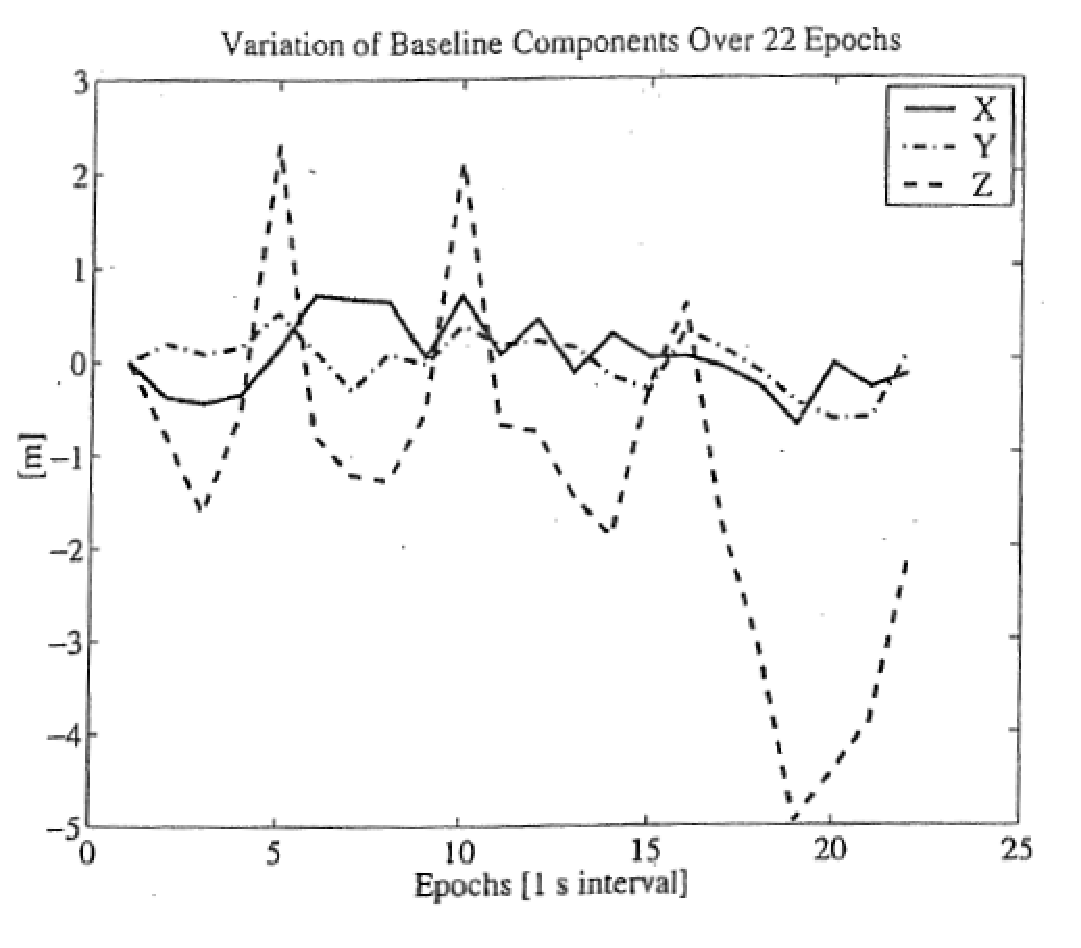
\includegraphics[width=0.4\linewidth]{TeX_files/Part03/chapter10/image/9-1}
	\caption{Baseline (X,Y,Z) over time,estimated from pseudoranges at two receivers}
	\label{fig:9-1}
\end{figure}

The standard deviation of phase noise e, as defined in (10.2), is a few millimeters,while the pseudorange error e depends on the quality of the receiver. C/A code pseudoranges can have noise values up to 2-3m, due to the slow chipping rate (which is another term for frequency). The P code arrives at 10.23 million binary digits or chips per second.This chipping rate is ten times higher than that of the C/A code and this implies a noise level of 10-30cm for the P code. A small pseudorange standard deviation is critical to quickly determining the integer ambiguities on LI or L2. The P code is normally encrypted, and then referred to as the Y code.

A short remark on how a dual frequency receiver works. Remember the C/A code is only transmitted on LI while the P code is transmitted on both LI and L2. The P codes are very long and they are not Gold codes. The receiver needs help to synchronize with the P code. That help comes from the C/A code and the data in the navigation message.The receiver synchronizes to the C/A code and demodulates the navigation message, quite analogous to a single frequency receiver. Within the message it finds data that describe the current contents of one of the shift registers used to generate the P code. With this help,P-code synchronization is accomplished. New technology now allows direct acquisition of P code or encrypted Y code. For further details see Misra \& Enge (2006).

This chapter is organized by

- Phase observations; the number N of waves is uncertain (ambiguity).

- Check of cycle slips; changes in the integer N .

- Differential GPS; two receivers.

- Double differences; two satellites and two receivers.

- Estimation of ambiguities; often also two frequencies.